\documentclass[11pt]{article}
\usepackage[margin=1in]{geometry}

%Set up packages
\usepackage{amsmath,amssymb,amsthm}
\usepackage{graphicx}
\usepackage{textcomp, gensymb}
\usepackage{float}
\usepackage{pdfpages}
\usepackage[hidelinks]{hyperref}
\usepackage{cancel}
\usepackage{subcaption}
\usepackage{caption}
 
\newcommand{\bm}{\boldsymbol}
\newcommand{\bI}{\mathbb{I}}
\newcommand{\bR}{\mathbb{R}}

\setlength\parindent{0pt}


\title{\bf OF-3 Report : \\[2mm] Simulating Supersonic Flow over a step}
\author{Terry Murray (tnm3843), Nicole Olvera (no4342), Andres Suniaga (aas5778)}
\date{04/10/2025}

\begin{document}
\maketitle

\noindent\makebox[\textwidth]{\rule{\textwidth}{0.2pt}}
\tableofcontents
\noindent\makebox[\textwidth]{\rule{\textwidth}{0.2pt}}
\pagebreak

\section{Introduction}
This report entails simluations of Mach 3 supersonic flow over a step as shown in Figure \ref{details}. We first take a walk through the equations that govern this flow such as a simplified \textit{Navier-Stokes} equations which make up Euler's equations and Normal Shock and Isentropic Flow theory. 


\begin{figure}[H]
    \centering
    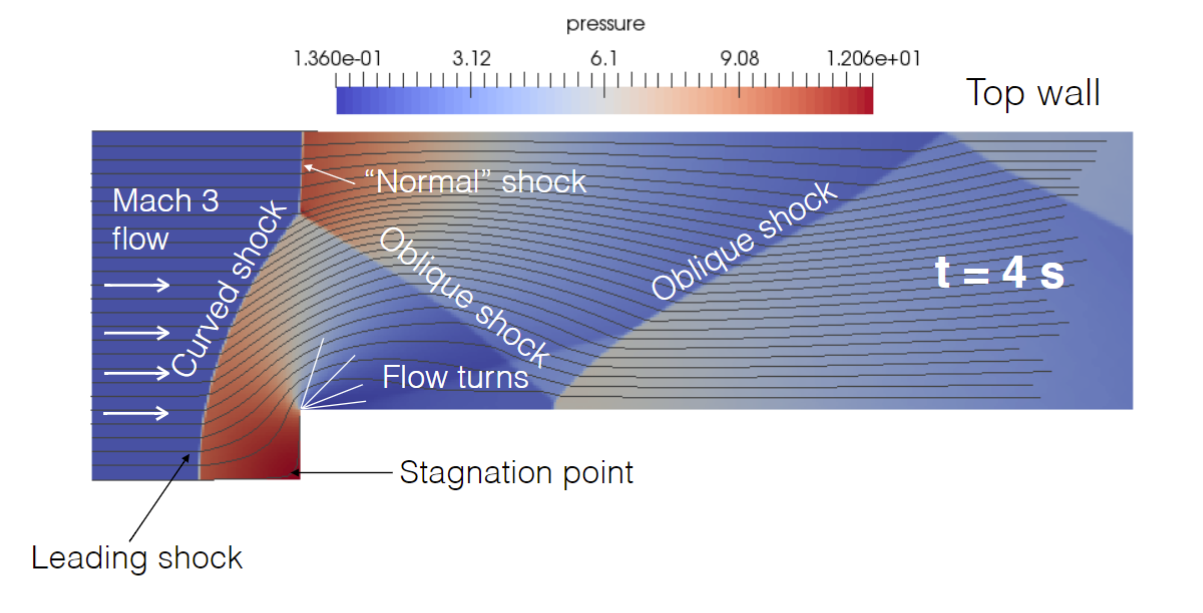
\includegraphics[width = 0.8\linewidth]{images/detailed_image_from_lecture.png}
    \caption{Details of the flow studied}
    \label{details}
\end{figure}
\vspace{2.5mm}

We then simulate this flow using \textit{OpenFoam's} \texttt{rhoCentralFoam} solver for various meshes from a coarse solution to more refined grids. \textit{Paraview} is used to visulaize the flow features such as the Mach number, velocity, temperature, pressure, and density. The stagnation point on the step is a point of interest as we compare the result of theory and CFD for the total pressure at this location. Lastly, we evaluate the performance of the parallel solver and observe how the number of processors affects the efficiency of the solver.

\pagebreak

\section{Governing Equations}
\subsection{Two-dimensional Euler equations}
We consider the Euler equations in $\bR^{2}$ complemented by the equation of state of an ideal gas (Eq. \ref{IGL}) with the specific heat ratio $\gamma = 1.4$. The two-dimensional Euler equations read:
\begin{equation}
   \frac{\partial \textbf{U}}{\partial t} + \frac{\partial \textbf{F}}{\partial x} + \frac{\partial \textbf{G}}{\partial y} = 0
\end{equation}

Where $\textbf{U}$ is the state vector, $\textbf{F}$ is the x-flux vector, and $\textbf{G}$ is the y-flux vector. 
\vspace{2.5mm}

From the assumptions of Euler equations, e.g., no body forces and inviscid and isothermal flow, the simplified form \textit{Navier-Stokes Equations} read:

\begin{itemize}
   \item Continuity : 
   \begin{equation}
       \frac{\partial \rho}{\partial t} + \rho \left(\frac{\partial u}{\partial x} + \frac{\partial v}{\partial y}\right) = 0 
   \end{equation}

   \item X-Momentum : 
   \begin{equation}
       \frac{\partial \rho \textbf{u}}{\partial t} + \rho \left(\frac{\partial u^{2}}{\partial x} + \frac{\partial uv}{\partial y}\right) = -\frac{\partial p}{\partial x}
   \end{equation}

   \item Y-Momentum : 
   \begin{equation}
       \frac{\partial \rho \textbf{v}}{\partial t} + \rho \left(\frac{\partial uv}{\partial x} + \frac{\partial v^2}{\partial y}\right) = -\frac{\partial p}{\partial y}
   \end{equation}

   \item Energy (inviscid simplification): 
   \begin{equation}
       \frac{\partial E}{\partial t} + E \left(\frac{\partial u}{\partial x} + \frac{\partial v}{\partial y}\right) = -p \left(\frac{\partial u}{\partial x} + \frac{\partial v}{\partial y}\right)
   \end{equation}

   Where \underline{$E = \rho (e + ||\bm{u}||^{2}/2)$}. $e$ is the internal energy of the fluid per unit mass (Joule per kilogram in SI).
\end{itemize}

Thus the state vector 
$\textbf{U} = 
\begin{bmatrix}
\rho \\[2mm]
\rho u \\[2mm]
\rho v \\[2mm]
\rho (e + \frac{1}{2}(u^{2}+v^{2}))    
\end{bmatrix} = \begin{bmatrix}
   \rho \\[2mm]
   \rho u \\[2mm]
   \rho v \\[2mm]
   E    
   \end{bmatrix}$.
\vspace{5mm}

The x-flux vector 
$\textbf{F} = 
\begin{bmatrix}
    \rho u \\[2mm]
    \rho u^{2} + p \\[2mm]
    \rho u v \\[2mm]
    (\rho (e + \frac{1}{2}(u^{2}+v^{2})) + p)* u
\end{bmatrix} = \begin{bmatrix}
   \rho u \\[2mm]
   \rho u^{2} + p \\[2mm]
   \rho u v \\[2mm]
   (E + p)(u)
\end{bmatrix}$
\vspace{5mm}

The y-flux vector
$\textbf{G} = 
\begin{bmatrix}
    \rho v \\[2mm]
    \rho v u \\[2mm]
    \rho v^2 + p \\[2mm]
    (\rho (e + \frac{1}{2}(u^{2}+v^{2})) + p)(v)
\end{bmatrix} = \begin{bmatrix}
   \rho v \\[2mm]
   \rho v u \\[2mm]
   \rho v^2 + p \\[2mm]
   (E + p)(v)
\end{bmatrix}$
\vspace{5mm}


The \textit{Ideal Gas Law} is our equation of state that relates the variables, $\rho$ which is our fluids density, $p$ the local pressure, $R$ the molecular gas constant, and $T$ the local temperature. 
\vspace{1mm}

\begin{equation}
   p = \rho RT 
   \label{IGL}
\end{equation}
\vspace{1.5mm}

Using the first law of Thermodynamics, $p$ can be related to the specific internal energy $e$ and the specific heat ratio $\gamma$ by:

\begin{equation}
   e = \frac{p}{\rho(\gamma-1)}
\end{equation}
\vspace{1.5mm}

These can be combined for a new expression that expresses \( p \) entirely in terms of the state vector \( \mathbf{U} \), allowing the flux vectors \( \mathbf{F(U)} \) and \( \mathbf{G(U)} \) to be evaluated directly from conserved quantities.
\vspace{1mm}

\begin{equation}
    p = (\gamma - 1)\left(E - \frac{1}{2} \rho (u^2 + v^2)\right)
\end{equation}
\vspace{2mm}


\subsection{Local Sound Speed and Mach Number}
To analyze compressible flow behavior, we often need the local sound speed and Mach number.
\vspace{2.5mm}

\textbf{Local Sound Speed:}

The local speed of sound \( a \) in a compressible fluid is given by the equation:

\begin{equation}
    a = \sqrt{\gamma R T} =\sqrt{\gamma \frac{p}{\rho}}
    \label{speedofsound}
\end{equation}

\textbf{Local Mach Number:}

The local Mach number \( M \) is defined as the ratio of the flow speed to the local speed of sound:

\begin{equation}
M = \frac{\sqrt{u^2 + v^2}}{a} = \frac{|\textbf{U}|}{a}
\label{Mach_equation}
\end{equation}

where \( u \) and \( v \) are the flow velocity components in the \( x \) and \( y \) directions, respectively.

\subsection{Normal Shock and Isentropic Flow Relations}
Here we look at the equations for normal shocks and isentropic flows,i.e., adiabatic and reversible.
\vspace{2.5mm}

For a normal shock with upstream (region 1) Mach number \(M_1\) and downstream (region 2) Mach number \(M_2\), the following standard jump conditions apply (for a perfect gas with ratio of specific heats \(\gamma\)):

\begin{itemize}
    \item \textbf{Static Pressure Ratio:}
    \begin{equation}
        \frac{p_2}{p_1} = 1 + \frac{2\,\gamma}{\gamma + 1} \bigl(M_1^2 - 1\bigr).
        \label{pressure_ratio}
    \end{equation}
    where:
    \begin{itemize}
        \item \( p_1 \): upstream (pre-shock) static pressure,
        \item \( p_2 \): downstream (post-shock) static pressure.
    \end{itemize}

    \item \textbf{Downstream Mach Number:}
    \begin{equation}
        M_2^2 = \frac{1 + \tfrac{\gamma - 1}{2}\,M_1^2}{\gamma\,M_1^2 - \tfrac{\gamma - 1}{2}}.
        \label{mach2equation}
    \end{equation}
\end{itemize}

Once the flow is on either side of a shock (and assuming no further shocks/viscous effects in that region), it can be treated as isentropic. In an isentropic flow of a perfect gas:
\begin{itemize}
    \item \textbf{Isentropic Pressure Relation: }
    \begin{equation}
      p_{0} = p\cdot(1+\dfrac{(\gamma - 1)}{2}M_{1}^{2})^{\frac{\gamma}{\gamma-1}}
      \label{isentropic_pressure}
   \end{equation}
   where:
   \begin{itemize}
       \item \( p_0 \): total (stagnation) pressure,
       \item \( p \): static pressure at a given point in the flow,
       \item \( M \): local Mach number at that point.
   \end{itemize}
\end{itemize}

\subsection{Step Example}
 Considering a flow over our step at $M=3$ and $p=1$ Pa, what is the pressure at the stagnation point (x=0.6m, y=0m in Figure \ref{overview}) on the surface of the step? We will employ the equations laid out above.
\vspace{2mm}

\begin{figure}[H]
   \centering
   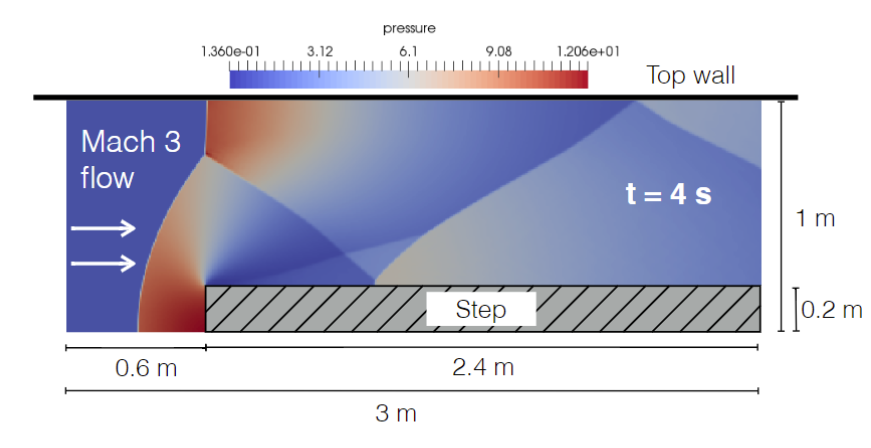
\includegraphics[width = 0.75\linewidth]{images/stepexample.png}
   \caption{Overview of the Flow}
   \label{overview}
\end{figure}


Using Equation \ref{isentropic_pressure} we can obtain the total pressure in the first region $p_{0_{1}} = 36.73\; \text{Pa}$. We can also obtain the local Mach past the shock using Equation \ref{mach2equation}, $M_{2} = 0.4752$. We can obtain our static pressure past the shock as $p_{2} =  p_{1}*\text{Eq. \ref{pressure_ratio}} = 10.33\; \text{Pa}$. Thus using Equation \ref{isentropic_pressure} again, we get a stagnation pressure $\boxed{p_{0_{2}} = 12.06\; \text{Pa}}$.

\pagebreak

\section{First Solution}
In this section we visualize the properties pressure $p$, density $\rho$, velocity $\textbf{U}$, and temperature $T$ after simulating Mach 3 flow over the step for $T=4\; \text{s}$.

\begin{figure}[H]
    \centering
    \begin{subfigure}{0.495\linewidth}
        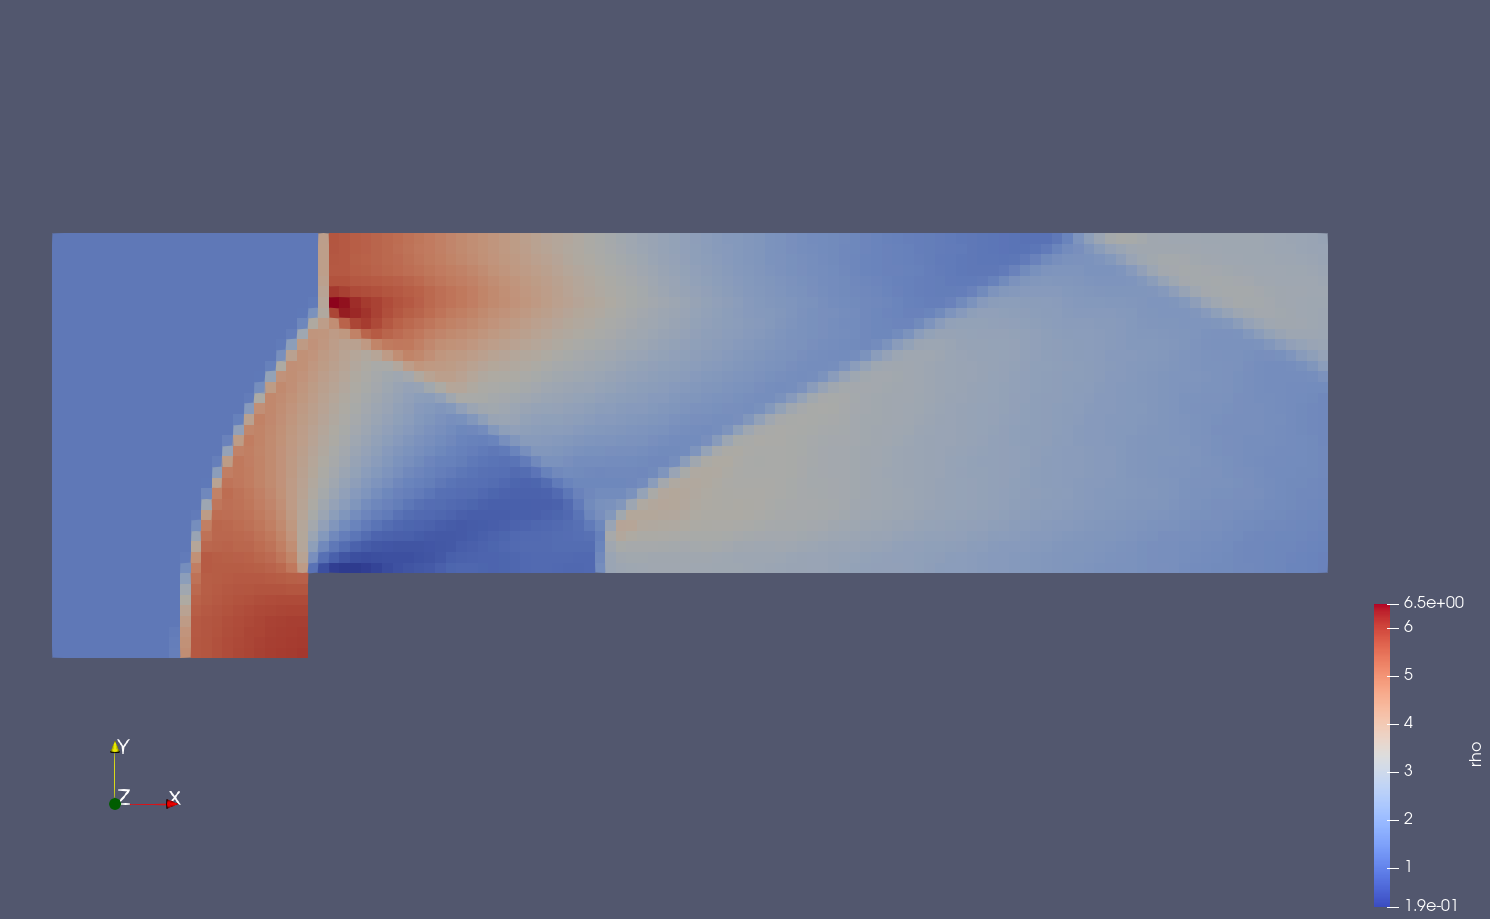
\includegraphics[width = \linewidth]{images/5_firstsolution_density.png}
        \caption{Density $\rho$}
    \end{subfigure}
    \begin{subfigure}{0.495\linewidth}
        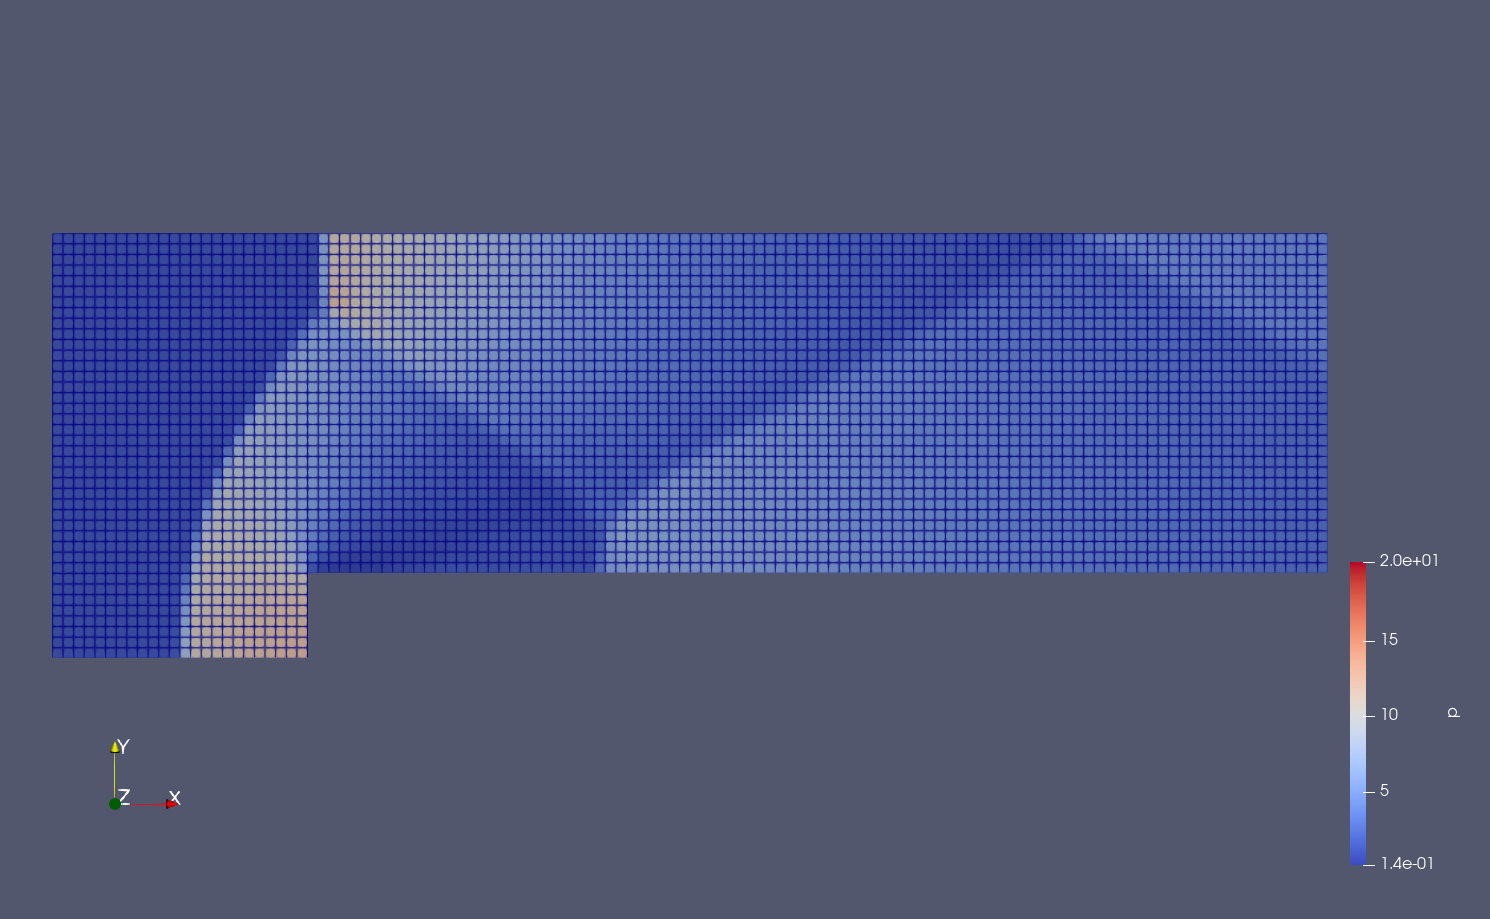
\includegraphics[width = \linewidth]{images/5_firstsolution_pressure.png}
        \caption{Pressure $p$}
    \end{subfigure}
    \vspace{2.5mm}

    \begin{subfigure}{0.495\linewidth}
        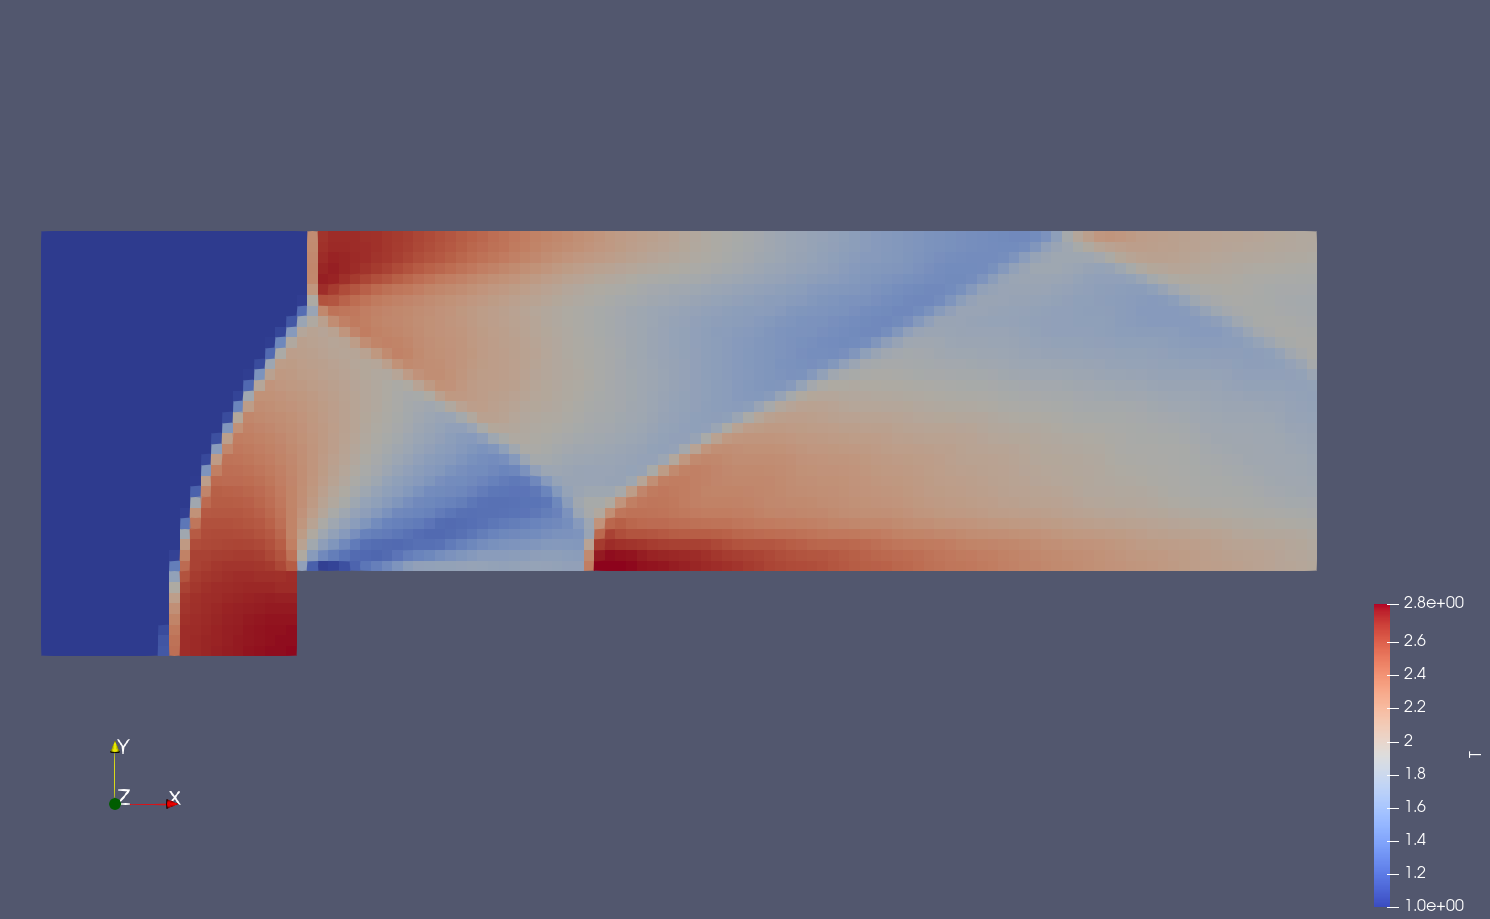
\includegraphics[width = \linewidth]{images/5_firstsolution_temperature.png}
        \caption{Temperature $T$}
    \end{subfigure}
    \begin{subfigure}{0.495\linewidth}
        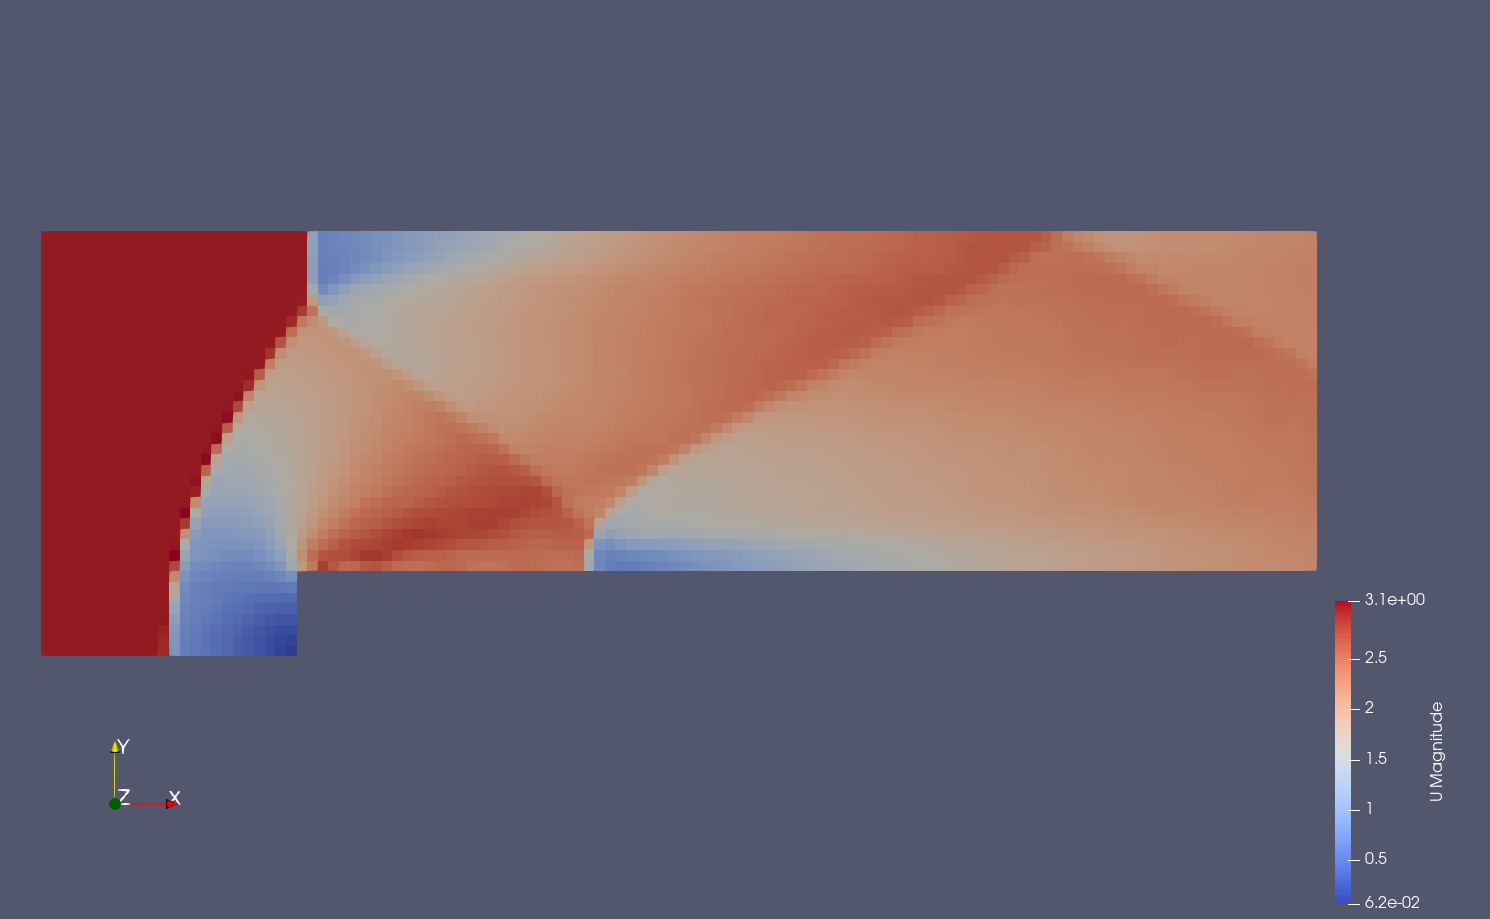
\includegraphics[width = \linewidth]{images/5_firstsolution_U_magnitude.png}
        \caption{Magnitude of Velocity $|\textbf{U}|$}
    \end{subfigure}
    \vspace{2.5mm}

    \begin{subfigure}{0.495\linewidth}
        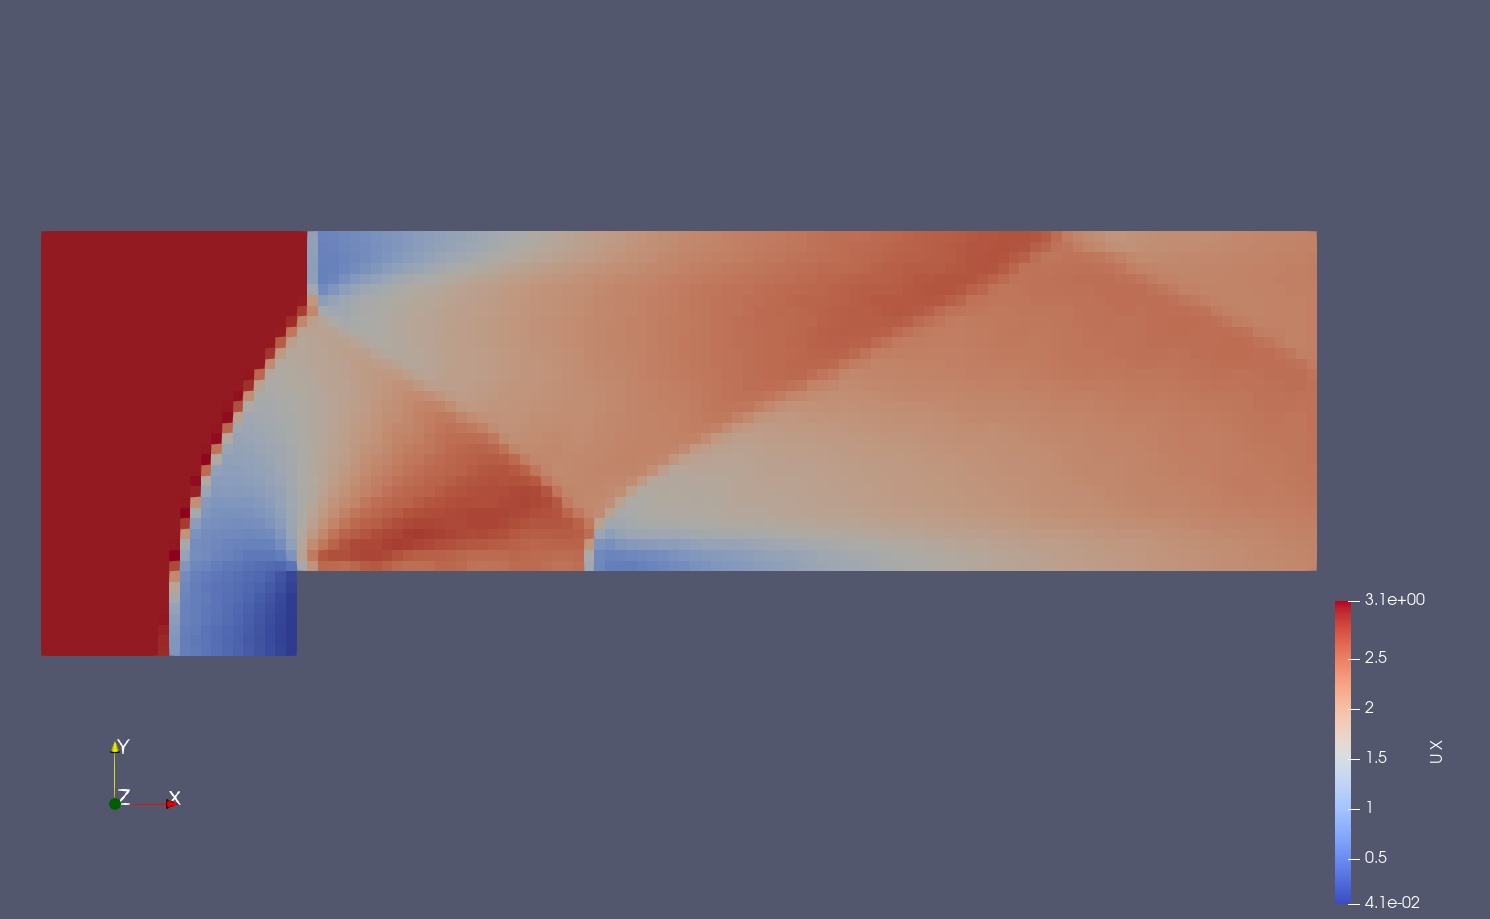
\includegraphics[width = \linewidth]{images/5_firstsolution_U_x.png}
        \caption{x-velocity $u$}
    \end{subfigure}
    \begin{subfigure}{0.495\linewidth}
        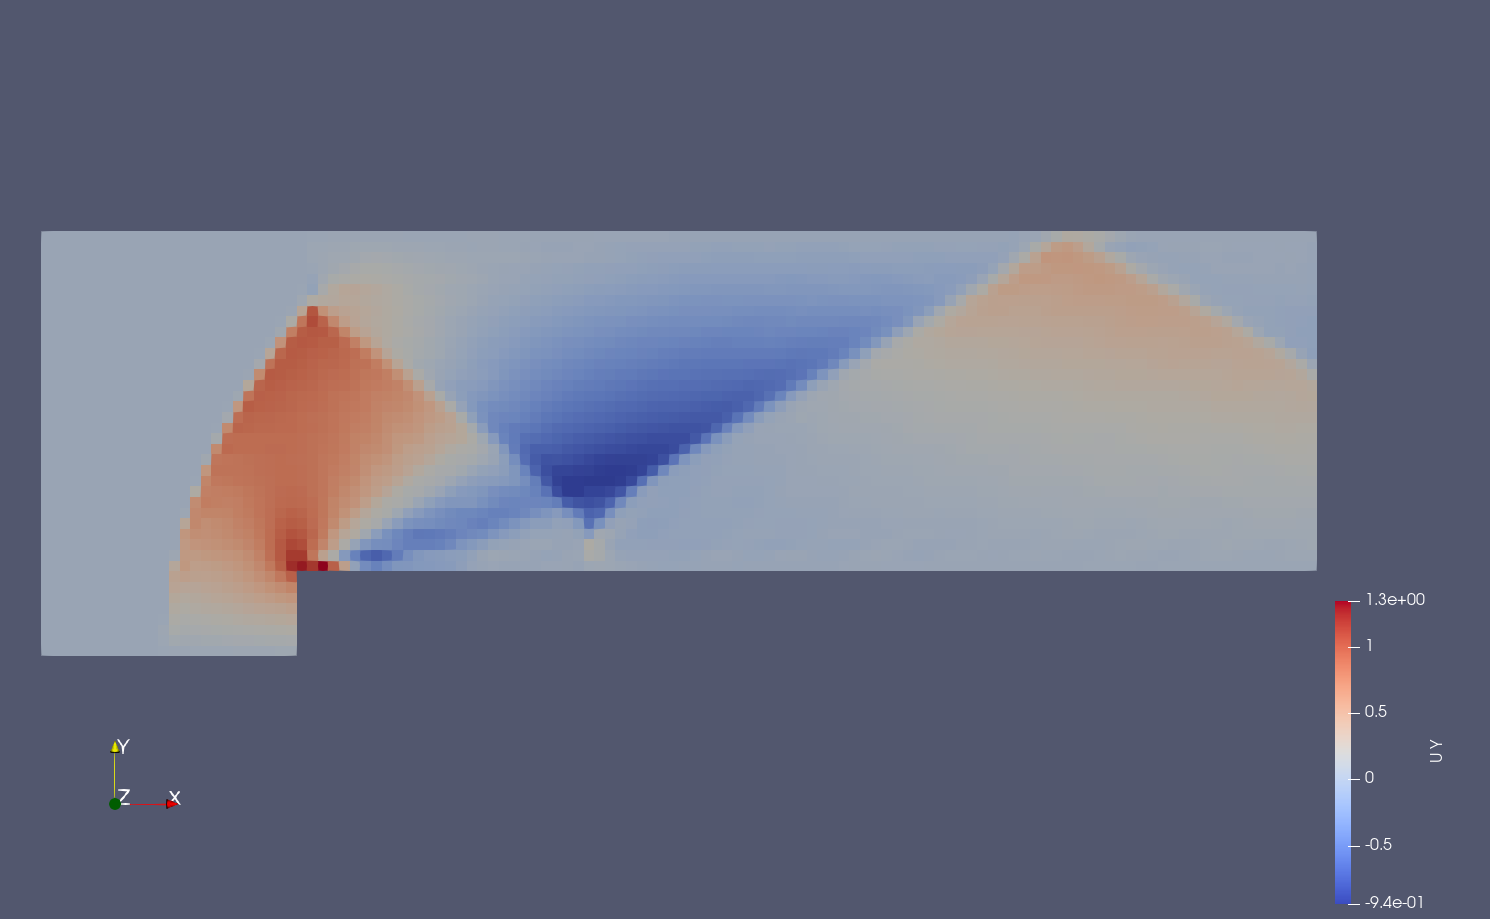
\includegraphics[width = \linewidth]{images/5_firstsolution_U_y.png}
        \caption{y-velocity $v$}
    \end{subfigure}
    \caption{Coarse mesh solution, gridpoints can be seen in the pressure plot}
    \label{coarsesolution}
\end{figure}
\vspace{5mm}

Using the built-in calculator in \textit{Paraview}, we are able to employ Equations \ref{speedofsound} and \ref{Mach_equation} to visulaize the Mach and Speed of Sound in our supersonic simulation.

\begin{figure}[H]
    \centering
    \begin{subfigure}{0.495\linewidth}
        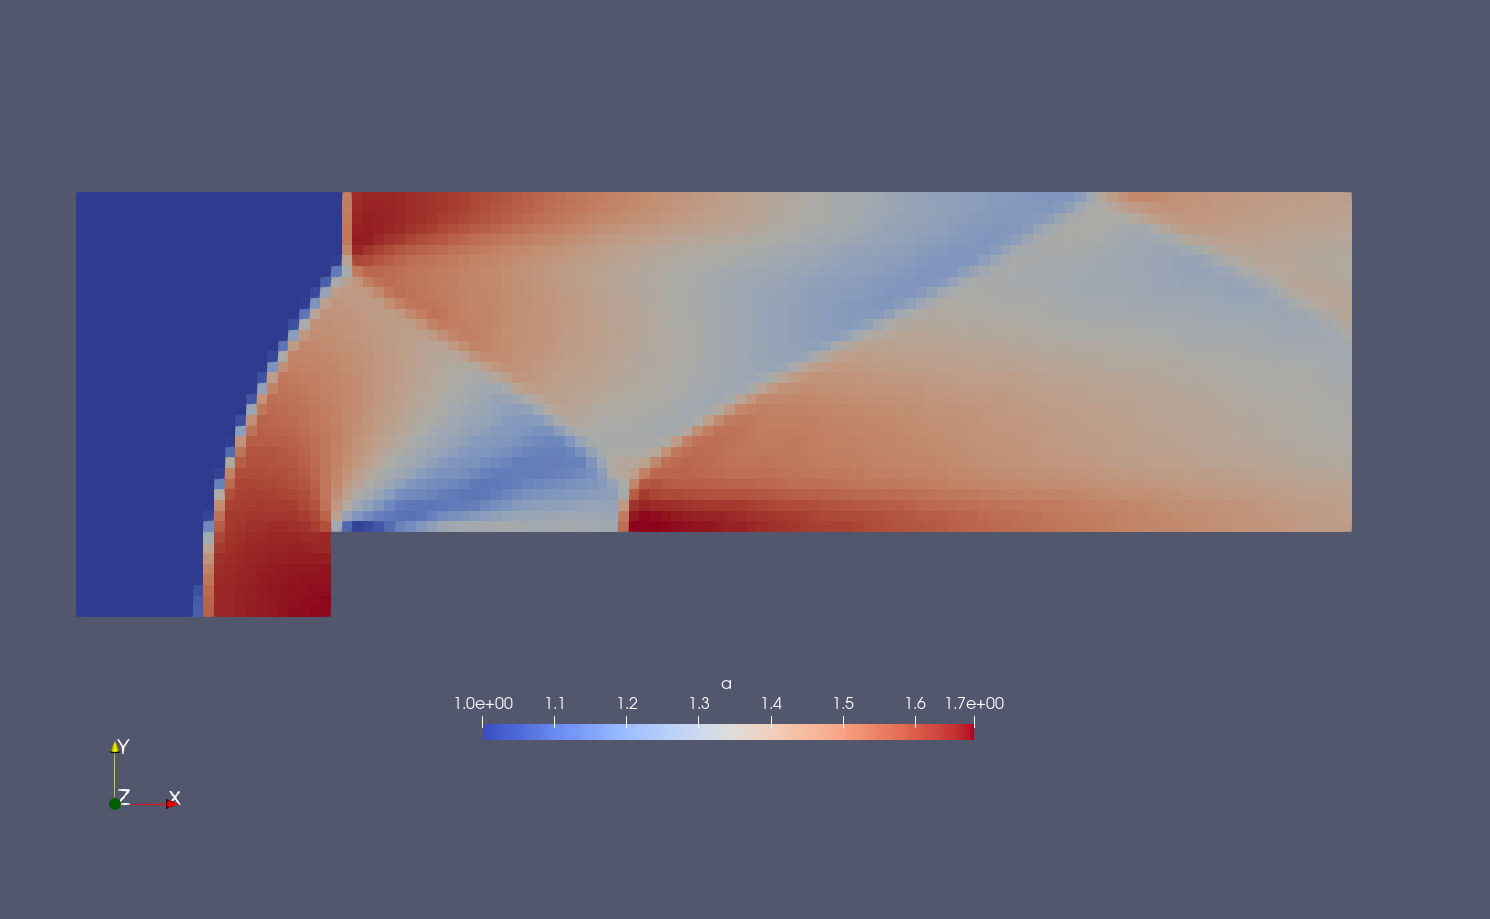
\includegraphics[width = \linewidth]{images/5_firstsolution_soundspeed.png}
        \caption{Speed of Sound $a$}
    \end{subfigure}    
    \begin{subfigure}{0.495\linewidth}
        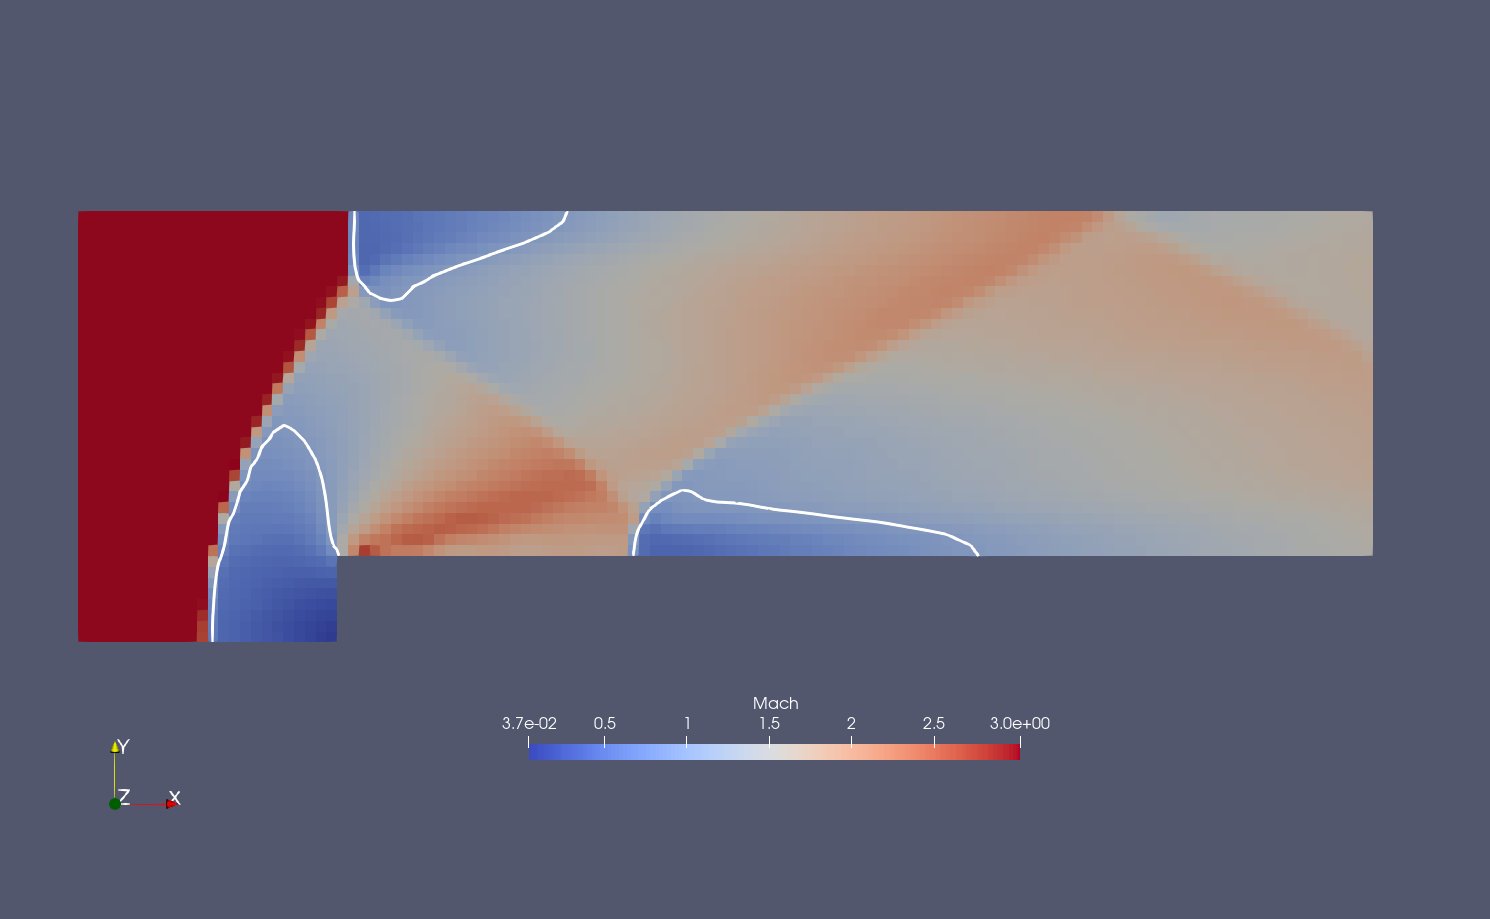
\includegraphics[width = \linewidth]{images/5_firstsolution_mach.png}
        \caption{Mach No. $M$}
    \end{subfigure}    
    \caption{White countour lines representing sonic flow, i.e., where $M=1$}
    \label{machandsoundspeed}
\end{figure}

The pressure at the stagnation grid point in this coarse mesh is $p = 11.9647\; \text{Pa}$. This is close but slightly less than what was computed using our normal shock theory.

\pagebreak

\section{Converging the Solution}

\pagebreak

\section{Parallel Solver Performance}
In this section, we analyze the performance characteristics of the parallel version of the \texttt{rhoCentralFoam} solver. The primary objective is to evaluate how effectively the solver scales when computing one simulation time step on different numbers of processors. Ideally, as we increase the number of processors, T(P), the time taken by the solver to advance one time step should decrease proportionally. We employ two critical performance metrics: parallel speedup and parallel efficiency.

Parallel speedup is defined as:

\begin{equation}
    \text{Speedup} = \frac{{T(1)}}{T(P)}
\end{equation}

where \(T(P)\) represents the computational time required by the solver advance the solution over one 
time step with \(P\) processors, and \(T(1)\) is the baseline computational time 
Parallel efficiency, \(\eta\), is defined as:

\begin{equation}
    \text{\(\eta\)} = \frac{{T(1)}}{T(P)}
\end{equation}

indicating how effecively processor resources are being utilized. 

We conducted scaling tests on a mesh of approximately one million cells, varying the number of processors from 1 up to 56 processors. The results of these scaling tests are summarized in Table \ref{table:performance} below, which lists the measured time step \(T(P)\), calculated parallel speedup, and parallel efficiency for each  tested processor \(P\).

\begin{table}[H]
    \centering
    \begin{tabular}{|c|c|c|c|}
        \hline
        \textbf{Processors (P)} & \textbf{Time \(T(P)\) [s]} & \textbf{Speedup} & \textbf{Efficiency (\(\eta\)) [\%]}\\
        \hline
        1 & 1.4183 & 1.0000 & 100.00 \\
        2 & 0.6595 & 2.1505 & 107.53 \\
        4 & 0.3357 & 4.2239 & 105.60 \\
        8 & 0.1764 & 8.0392 & 100.49 \\
        16 & 0.1061 & 13.3668 & 85.54 \\
        32 & 0.0663 & 21.3712 & 66.79 \\
        56 & 0.0529 & 26.8098 & 47.87 \\
        \hline
    \end{tabular}
    \caption{Parallel Performance Metrics for \texttt{rhoCentralFoam} Solver for Different \# of Processors}
    \label{table:performance}
\end{table}

\begin{figure}[H]
    \centering
    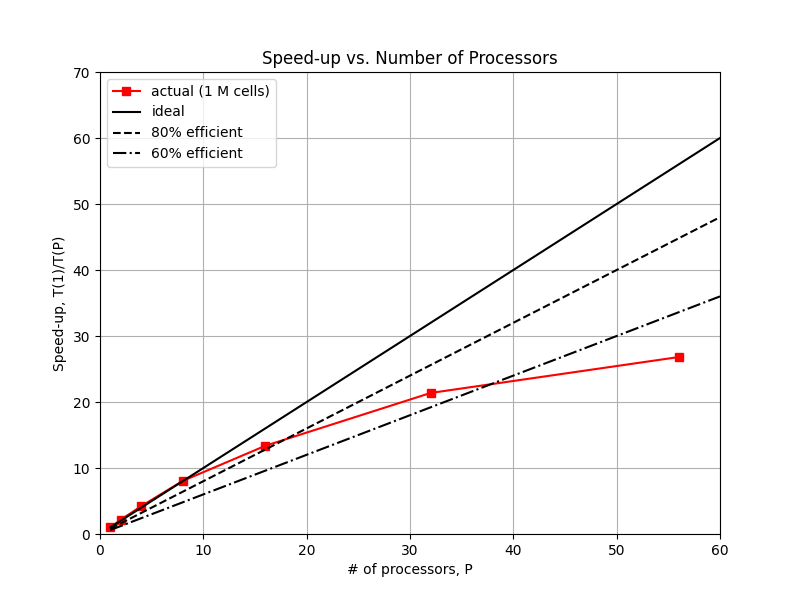
\includegraphics[width=0.7\textwidth]{images/speedup_vs_processors.png}
    \caption{Speedup vs. Number of Processors \(P\).}
    \label{fig:speedup}
\end{figure}

The collected data and graph clearly demonstrate that initially, as the number of processors increases, the speedup closely follows the ideal linear scaling. 

\pagebreak
\appendix
\pagenumbering{gobble} 
\begin{center}
\vspace*{\fill}
   \Huge \bf Appendix 
\vspace*{\fill}
\end{center}
\pagebreak 

\hypertarget{code}{}
\section{Code}
PDF of code starts on next page. 
\vspace{2.5mm}

Additionally, team repository: \url{https://github.com/andressuniaga/CFD-SP25-11}

% \includepdf[pages=-]{}

\end{document}